\let\lesson\undefined
\newcommand{\lesson}{\phantomlesson{Bài 4.}}
\setcounter{section}{2}
\section{Bài tập trắc nghiệm}
\begin{enumerate}[label=\bfseries Câu \arabic*:]
	\item \mkstar{2}\\
	{\begin{minipage}[l]{0.7\textwidth}
			Cho đồ thị độ dịch chuyển – thời gian của một vật như hình. Chọn phát biểu đúng.
			\begin{mcq}
				\item Vật đang chuyển động thẳng đều theo chiều dương.
				\item Vật đang chuyển động thẳng đều theo chiều âm.
				\item Vật đang đứng yên.
				\item Vật chuyển động thẳng đều theo chiều dương rồi đổi chiều chuyển động ngược lại.
			\end{mcq}
		\end{minipage}
		\begin{minipage}{0.3\textwidth}
			\begin{center}
				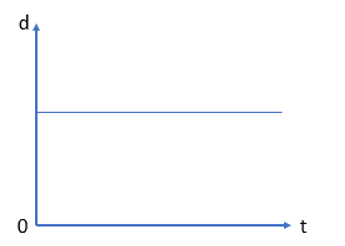
\includegraphics[width=0.9\linewidth]{../figs/VN10-2023-PH-TP005-P-1}
			\end{center}
		\end{minipage}
}
\hideall{
\textbf{Đáp án: C.}
}

\item \mkstar{2}\\
{\begin{minipage}[l]{0.7\textwidth}
		Cho đồ thị độ dịch chuyển – thời gian của một vật như hình. Chọn phát biểu đúng.
		\begin{mcq}
			\item Vật đang chuyển động thẳng đều theo chiều dương.
			\item Vật đang chuyển động thẳng đều theo chiều âm.
			\item Vật đang đứng yên.
			\item Vật chuyển động thẳng đều theo chiều dương rồi đổi chiều chuyển động ngược lại.
		\end{mcq}
	\end{minipage}
	\begin{minipage}{0.3\textwidth}
		\begin{center}
			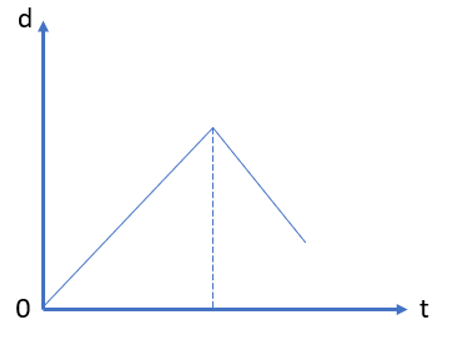
\includegraphics[width=0.9\linewidth]{../figs/VN10-2023-PH-TP005-P-2}
		\end{center}
	\end{minipage}
}
\hideall{
	\textbf{Đáp án: D.}
}

\item \mkstar{2}\\
{Cho đồ thị độ dịch chuyển – thời gian trong chuyển động thẳng của một xe ô tô đồ chơi điều khiển từ xa.\\
	\begin{minipage}[l]{0.6\textwidth}
		Chọn kết luận \textbf{sai}.
		\begin{mcq}
			\item Trong 2 giây đầu xe chuyển động vói vận tốc không đổi.
			\item Từ giây thứ 2 đến giây thứ 4 xe dừng lại.
			\item Từ giây thứ 4 đến giây thứ 9 xe đổi chiều chuyển động theo hướng ngược lại với tốc độ nhỏ hơn lúc đi.
			\item Từ giây thứ 9 đến giây thứ 10 xe quay về đúng vị trí xuất phát rồi dừng lại.
		\end{mcq}
	\end{minipage}
\begin{minipage}{0.4\textwidth}
	\begin{center}
		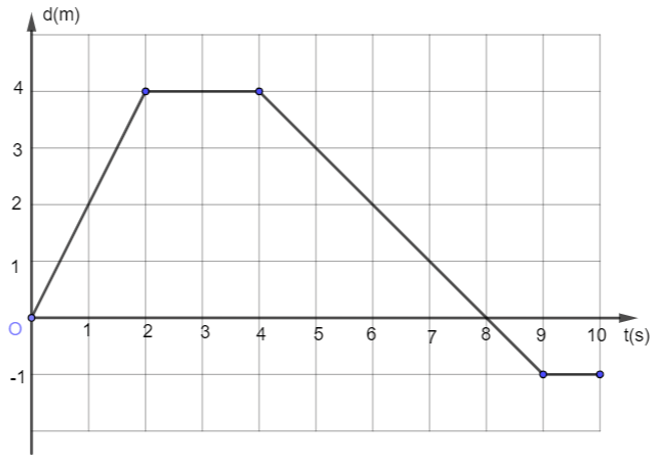
\includegraphics[width=1.0\linewidth]{../figs/VN10-2023-PH-TP005-P-3}
	\end{center}
\end{minipage}
}
\hideall{
\textbf{Đáp án: D.}
}

\item \mkstar{2}\\
{\begin{minipage}[l]{0.7\textwidth}
		Đồ thị độ dịch chuyển – thời gian trong chuyển động thẳng của một chất điểm có dạng như hình vẽ.\\
		Trong thời gian nào xe chuyển động thẳng đều?
		\begin{mcq}
			\item Trong khoảng thời gian từ $0$ đến $t_1$.
			\item Trong khoảng thời gian từ $0$ đến $t_2$.
			\item Trong khoảng thời gian từ $t_1$ đến $t_2$.
			\item Không có lúc nào xe chuyển động thẳng đều.
		\end{mcq}
	\end{minipage}
\begin{minipage}{0.3\textwidth}
	\begin{center}
		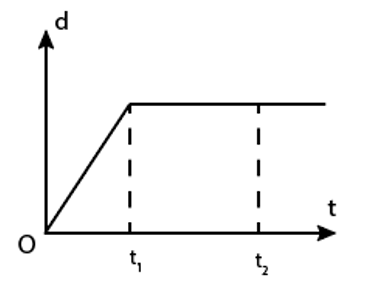
\includegraphics[width=0.8\linewidth]{../figs/VN10-2023-PH-TP005-P-4}
	\end{center}
\end{minipage}
}
\hideall{
\textbf{Đáp án: A.}
}

\item \mkstar{2}\\
{Phương trình chuyển động của một chất điểm dọc theo trục $Ox$ có dạng: $x = 5 + 60t$ ($x$ đo bằng kilomét và $t$ đo bằng giờ). Chất điểm đó xuất phát từ điểm nào và chuyển động với vận tốc bằng bao nhiêu?
	\begin{mcq}
		\item Từ điểm $O$, với vận tốc $\SI{5}{\kilo\meter/\hour}$.
		\item Từ điểm $O$, với vận tốc $\SI{60}{\kilo\meter/\hour}$.
		\item Từ điểm $M$ cách $O$ $\SI{5}{\kilo\meter/\hour}$, với vận tốc $\SI{5}{\kilo\meter/\hour}$.
		\item Từ điểm $M$ cách $O$ $\SI{5}{\kilo\meter/\hour}$, với vận tốc $\SI{60}{\kilo\meter/\hour}$.
	\end{mcq}

}
\hideall{
\textbf{Đáp án: D.}
}

\item \mkstar{2}\\
{Phương trình chuyển động của một chất điểm dọc theo $Ox$ có dạng: $x=5t-12$ (km), với $t$ đo bằng giờ. Độ dời của chất điểm từ $\SI{2}{\hour}$ đến $\SI{4}{\hour}$ là
\begin{mcq}(4)
	\item $\SI{8}{\kilo\meter}$.
	\item $\SI{6}{\kilo\meter}$.
	\item $\SI{10}{\kilo\meter}$.
	\item $\SI{2}{\kilo\meter}$.
\end{mcq}
}
\hideall{
\textbf{Đáp án: C.}
}

\item \mkstar{2}\\
{Phương trình chuyển động của một chất điểm dọc theo trục $Ox$ có dạng: $x = 4 -10t$ ($x$ đo bằng kilomét và $t$ đo bằng giờ). Quãng đường đi được của chất điểm sau $\SI{2}{\hour}$ chuyển động là
	\begin{mcq}(4)
		\item $\SI{-20}{\kilo\meter}$.
		\item $\SI{20}{\kilo\meter}$.
		\item $\SI{-8}{\kilo\meter}$.
		\item $\SI{8}{\kilo\meter}$.
	\end{mcq}
}
\hideall{
\textbf{Đáp án: B.}
}





\item \mkstar{3}\\
{\begin{minipage}[l]{0.6\textwidth}
		Hình vẽ bên là đồ thị độ dịch chuyển - thời gian của một chiếc xe ô tô chạy từ $A$ đến $B$ trên một đường thẳng. Vận tốc của xe bằng
		\begin{mcq}
			\item $\SI{30}{\kilo\meter/\hour}$.
			\item $\SI{150}{\kilo\meter/\hour}$.
			\item $\SI{120}{\kilo\meter/\hour}$.
			\item $\SI{100}{\kilo\meter/\hour}$.
		\end{mcq}
	\end{minipage}
\begin{minipage}{0.4\textwidth}
		\begin{center}
			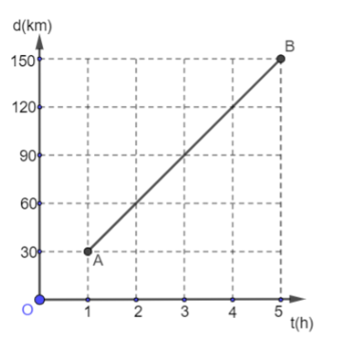
\includegraphics[width=0.6\linewidth]{../figs/VN10-2023-PH-TP005-P-5}
		\end{center}
	\end{minipage}
}
\hideall{
\textbf{Đáp án: A.}
}


\item \mkstar{3}\\
{\begin{minipage}[l]{0.6\textwidth}
		Đồ thị độ dịch chuyển – thời gian của một vật chuyển động như hình vẽ. Vật chuyển động
		\begin{mcq}
			\item ngược chiều dương với tốc độ $\SI{20}{\kilo\meter/\hour}$.
			\item cùng chiều dương với tốc độ $\SI{20}{\kilo\meter/\hour}$.
			\item ngược chiều dương với tốc độ $\SI{60}{\kilo\meter/\hour}$.
			\item cùng chiều dương với tốc độ $\SI{60}{\kilo\meter/\hour}$.
		\end{mcq}
	\end{minipage}
	\begin{minipage}{0.4\textwidth}
		\begin{center}
			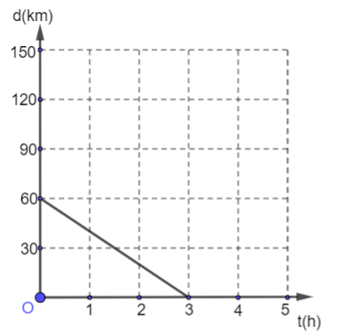
\includegraphics[width=0.6\linewidth]{../figs/VN10-2023-PH-TP005-P-6}
		\end{center}
	\end{minipage}
}
\hideall{
	\textbf{Đáp án: A.}
}

\item \mkstar{3}\\
{\begin{minipage}[l]{0.7\textwidth}
		Một chất điểm chuyển động trên một đường thẳng. Đồ thị độ dịch chuyển theo thời gian của chất điểm được mô tả như hình vẽ. Tốc độ trung bình của chất điểm trong khoảng thời gian từ 0 đến $\SI{5}{\second}$ là
		\begin{mcq}(2)
			\item $\SI{1.6}{\centi\meter/\second}$.
			\item $\SI{6.4}{\centi\meter/\second}$.
			\item $\SI{4.8}{\centi\meter/\second}$.
			\item $\SI{2.4}{\centi\meter/\second}$.
		\end{mcq}
	\end{minipage}
	\begin{minipage}{0.3\textwidth}
		\begin{center}
			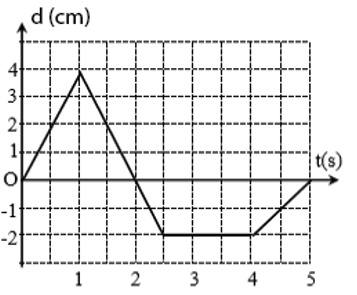
\includegraphics[width=0.8\linewidth]{../figs/VN10-2023-PH-TP005-P-7}
		\end{center}
	\end{minipage}
}
\hideall{
	\textbf{Đáp án: D.}
}

\item \mkstar{3}\\
{Một người đi bằng thuyền với tốc độ $\SI{2}{\meter/\second}$ về phía đông. Sau khi đi được $\SI{2.2}{\kilo\meter}$, người này lên ô tô đi về phía bắc trong 15 phút với tốc độ $\SI{60}{\kilo\meter/\hour}$. Hãy chọn kết luận \textbf{sai}.
	\begin{mcq}(2)
		\item Tổng quãng đường đã đi là $\SI{17.2}{\kilo\meter}$.
		\item Độ dịch chuyển là $\SI{15.2}{\kilo\meter}$.
		\item Tốc độ trung bình là $\SI{8.6}{\meter/\second}$.
		\item Vận tốc trung bình bằng $\SI{8.6}{\meter/\second}$.
	\end{mcq}
}
\hideall{
	\textbf{Đáp án: B.}
}

\item \mkstar{3}\\
{Một người bơi dọc theo chiều dài $\SI{100}{\meter}$ của bể bơi hết $\SI{60}{\second}$ rồi quay về lại chỗ xuất phát trong $\SI{70}{\second}$. Trong suốt quãng đường đi và về tốc độ trung bình, vận tốc trung bình của người đó lần lượt là
\begin{mcq}(4)
	\item $\SI{1.538}{\meter/\second}$; $\SI{0}{\meter/\second}$.
	\item $\SI{1.538}{\meter/\second}$; $\SI{1.876}{\meter/\second}$.
	\item $\SI{3.077}{\meter/\second}$; $\SI{2}{\meter/\second}$.
	\item $\SI{7.692}{\meter/\second}$; $\SI{2.2}{\meter/\second}$.
\end{mcq}
}
\hideall{
\textbf{Đáp án: A.}
}


\item \mkstar{3}\\
{Lúc $\SI{7}{\hour}$, ô tô thứ nhất đi qua điểm $A$, ô tô thứ hai đi qua điểm $B$ cách $A$ $\SI{10}{\kilo\meter}$. Xe đi qua $A$ với vận tốc $\SI{50}{\kilo\meter/\hour}$, xe đi qua $B$ với vận tốc $\SI{40}{\kilo\meter/\hour}$. Biết hai xe chuyển động cùng chiều theo hướng từ $A$ đến $B$. Coi chuyển động của 2 ô tô là chuyển động đều. Hỏi
\begin{enumerate}[label=\alph*)]
	\item Hai xe gặp nhau lúc mấy giờ?
	\begin{mcq}(4)
		\item 7h30.
		\item 8h.
		\item 9h.
		\item 8h30.
	\end{mcq}
\item Quãng đường xe $A$ đã đi được đến khi gặp xe $B$ là
\begin{mcq}(4)
	\item $\SI{80}{\kilo\meter}$.
	\item $\SI{40}{\kilo\meter}$.
	\item $\SI{50}{\kilo\meter}$.
	\item $\SI{90}{\kilo\meter}$.
\end{mcq}
\item Hai xe cách nhau 20 km lúc mấy giờ?
\begin{mcq}(4)
	\item 9h.
	\item 9h30.
	\item 10h.
	\item 11h.
\end{mcq}
\end{enumerate}
}
\hideall{
\textbf{Đáp án: B - C - C.}
}

\item \mkstar{3}\\
{Hãy viết phương trình chuyển động của một ô tô chuyển động thẳng đều biết rằng tại $t_1=\SI{2}{\hour}$ thì $x_1=\SI{40}{\kilo\meter}$ và tại $t_2 =\SI{3}{\hour}$ thì $x_2=\SI{90}{\kilo\meter}$.
	\begin{mcq}(4)
		\item $x=-60+50t\qquad\left(\si{\kilo\meter}, \si{\hour}\right)$.
		\item $x=-60+30t\qquad\left(\si{\kilo\meter}, \si{\hour}\right)$.
		\item $x=-60+40t\qquad\left(\si{\kilo\meter}, \si{\hour}\right)$.
		\item $x=-60+20t\qquad\left(\si{\kilo\meter}, \si{\hour}\right)$.
	\end{mcq}
}
\hideall{
\textbf{Đáp án: A.}
}

\item \mkstar{3}\\
{Hãy thiết lập phương trình chuyển động của một ô tô chuyển động thẳng đều biết. Ôtô chuyển động theo chiều dương với vận tốc $\SI{10}{\meter/\second}$ và ở thời điểm $\SI{3}{\second}$ thì ô tô có tọa độ $\SI{60}{\meter}$.
\begin{mcq}(4)
	\item $x=30+10t\qquad\left(\si{\meter}, \si{\second}\right)$.
	\item $x=20+10t\qquad\left(\si{\meter}, \si{\second}\right)$.
	\item $x=10+20t\qquad\left(\si{\meter}, \si{\second}\right)$.
	\item $x=40+10t\qquad\left(\si{\meter}, \si{\second}\right)$.
\end{mcq}
}
\hideall{
\textbf{Đáp án: A.}}

\item \mkstar{3}\\
{Hai trạm dừng chân $A$ và $B$ cách nhau $\SI{72}{\kilo\meter}$. Lúc 7h30 sáng, xe ô tô 1 khởi hành từ $A$ chuyển động thẳng đều về $B$ với tốc độ $\SI{36}{\kilo\meter/\hour}$. Nửa giờ sau, xe ô tô 2 chuyển động thẳng đều từ $B$ đến $A$ và gặp ô tô 1 lúc 8 giờ 30 phút. Tìm tốc độ của xe ô tô thứ hai.
	\begin{mcq}(4)
		\item $v_2=\SI{70}{\kilo\meter/\hour}$.
		\item $v_2=\SI{72}{\kilo\meter/\hour}$.
		\item$v_2=\SI{73}{\kilo\meter/\hour}$.
		\item $v_2=\SI{74}{\kilo\meter/\hour}$.
	\end{mcq}

}
\hideall{
\textbf{Đáp án: B.}
}

\item \mkstar{3}\\
{Lúc 7 giờ một người đang ở $A$ chuyển động thẳng đều với vận tốc $\SI{10}{\meter/\second}$ đuổi theo người ở $B$ đang chuyển động thẳng đều với vận tốc $\SI{18}{\kilo\meter/\hour}$. Biết $AB =\SI{36}{\kilo\meter}$. Chọn trục tọa độ trùng với quỹ đạo chuyển động, chiều dương là chiều chuyển động, gốc tọa độ tại A, gốc thời gian là lúc $\SI{7}{\hour}$. Thời điểm và vị trí người thứ nhất đuổi kịp người thứ hai là
\begin{mcq}(2)
	\item lúc $\SI{2}{\hour}$ cách $A$ $\SI{72}{\kilo\meter}$.
	\item lúc $\SI{9}{\hour}$ cách $B$ $\SI{36}{\kilo\meter}$.
	\item lúc $\SI{9}{\hour}$ cách $A$ $\SI{72}{\kilo\meter}$.
	\item lúc $\SI{2}{\hour}$ cách $B$ $\SI{36}{\kilo\meter}$.
\end{mcq}
}
\hideall{
\textbf{Đáp án: C.}
}

\item \mkstar{3}\\
{Lúc $\SI{10}{\hour}$ có một xe xuất phát từ $A$ đi về $B$ với tốc độ $\SI{50}{\kilo\meter/\hour}$. Lúc 10h30 một xe khác xuất phát từ $B$ đi về $A$ với tốc độ $\SI{80}{\kilo\meter/\hour}$. Cho $AB =\SI{200}{\kilo\meter}$. Lúc $\SI{11}{\hour}$, hai xe cách nhau
\begin{mcq}(4)
	\item $\SI{100}{\kilo\meter}$.
	\item $\SI{110}{\kilo\meter}$.
	\item $\SI{150}{\kilo\meter}$.
	\item $\SI{160}{\kilo\meter}$.
\end{mcq}
}
\hideall{
\textbf{Đáp án: B.}
}

\item \mkstar{4}\\
{\begin{minipage}[l]{0.7\textwidth}
		Hình dưới là đồ thị độ dịch chuyển - thời gian của hai vật chuyển động thẳng cùng hướng. Tỉ lệ vận tốc $\dfrac{v_A}{v_B}$ là
		\begin{mcq}(2)
			\item $\dfrac{3}{1}$.
			\item $\dfrac{1}{3}$.
			\item $\dfrac{\sqrt{3}}{1}$.
			\item $\dfrac{1}{\sqrt{3}}$.
		\end{mcq}
	\end{minipage}
	\begin{minipage}{0.3\textwidth}
		\begin{center}
			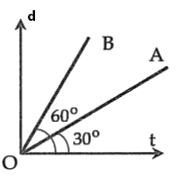
\includegraphics[width=0.7\linewidth]{../figs/VN10-2023-PH-TP005-P-8}
		\end{center}
	\end{minipage}
}
\hideall{
	\textbf{Đáp án: B.}
}


\end{enumerate}
\section{Bài tập tự luận}
\begin{enumerate}[label=\bfseries Bài \arabic*:]
	\item \mkstar{3}
	
	
	{
		Bạn A đi học từ nhà đến trường theo lộ trình ABC. Biết bạn A đi đoạn đường $\text{AB} = \SI{400}{m}$ hết 6 phút, đoạn đường $\text{BC} = \SI{300}{m}$ hết 4 phút. Xác định tốc độ trung bình và vận tốc trung bình của bạn A khi đi từ nhà đến trường.
		\begin{center}
			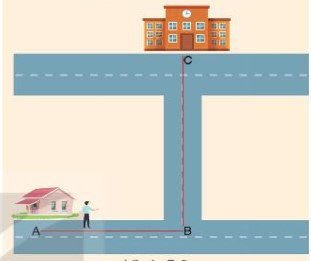
\includegraphics[scale=1]{../figs/VN10-2022-PH-TP005-2.jpg}
		\end{center}
	}
	\hideall
	{
		Độ dịch chuyển của bạn A đến trường chính là độ dài
		
		$$\text{AB} = \sqrt{(\text{AB})^2 + (\text{BC})^2} = \SI{500}{m}.$$
		
		Tốc độ trung bình 
		
		$$v= \dfrac{s}{t} = \dfrac{300+400}{(6 + 4)60}  = \SI{1,17}{m/s}.$$
		
		Vận tốc trung bình
		
		$$v'=\dfrac{d}{t}=\dfrac{500}{(6+4)60} = \SI{0,83}{m/s}.$$
	}

	\item \mkstar{2}
	
	{
		Hãy vẽ đồ thị độ dịch chuyển - thời gian trong chuyển động của A theo bảng ghi số liệu vào vở. Trên trục tung (trục độ dịch chuyển) $\SI{1}{cm}$ ứng với $\SI{200}{m}$; trên trục hoành (trục thời gian) $\SI{1}{cm}$ ứng với $\SI{50}{s}$.
		
		\begin{center}
			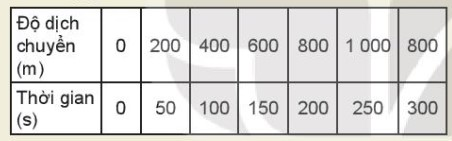
\includegraphics[scale=1]{../figs/VN10-2022-PH-TP006-5.jpg}
		\end{center}
		
	}
	\hideall{
		
		Từ bảng số liệu ta vẽ được đồ thị như hình sau:
		
		
		\begin{center}
			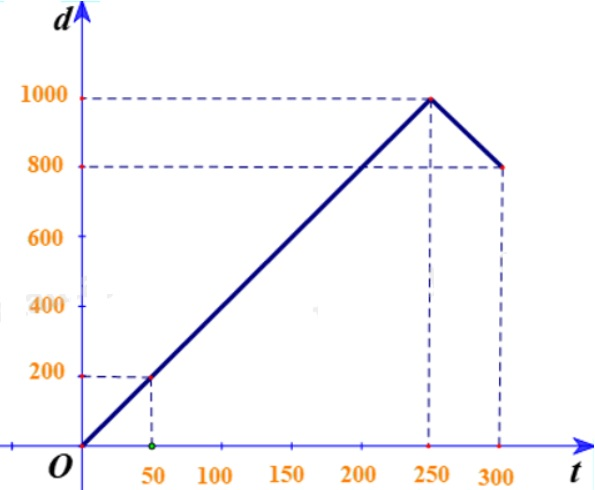
\includegraphics[scale=0.6]{../figs/VN10-2022-PH-TP006-6.jpg}
		\end{center}
		
	}
	

	\item \mkstar{3}
	
	{
		Đồ thị độ dịch chuyển - thời gian của một người đang bơi trong một bể bơi dài $\SI{50}{m}$. 
		\begin{center}
			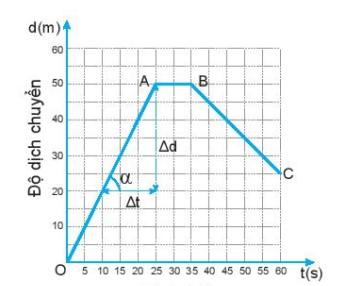
\includegraphics[scale=1]{../figs/VN10-2022-PH-TP006-2.jpg}
		\end{center}
	\begin{enumerate}[label=\alph*)]
		\item Trong 25 giây đầu mỗi giây người đó bơi được bao nhiêu mét? Tính vận tốc của người đó ra m/s. Từ giây nào đến giây nào người đó không bơi?
		\item Từ giây 35 đến giây 60 người đó bơi theo chiều nào? Trong 20 giây cuối cùng, mỗi giây người đó bơi được bao nhiêu mét? Tính vận tốc của người đó ra m/s.
		\item Xác định độ dịch chuyển và vận tốc của người đó trong cả quá trình bơi.
	\end{enumerate}
}
	\hideall{
		\begin{enumerate}[label=\alph*)]
			\item Từ đồ thị ta thấy, trong 25 giây đầu người đó chuyển động thẳng từ O – A và không đổi chiều, độ dịch chuyển trong 25 giây đầu là $\SI{50}{m}$.
			
			Mỗi giây người đó bơi được:
			
			$$\dfrac{50}{25} = \SI{2}{m}.$$
			
			Vận tốc của người đó:
			
			$$v = \dfrac{d}{t} = \dfrac{50}{25} = \SI{2}{m/s}.$$
			
			Từ A – B: người đó không bơi $\Rightarrow$ Người đó không bơi từ giây 25 đến giây 35.
			\item Từ giây 35 đến giây 60 người đó bơi ngược chiều dương.
			
			Trong 20 giây cuối cùng:
			
			Từ đồ thị ta thấy
			\begin{itemize}
				\item Giây thứ 40 có $d_1 = \SI{45}{m}$.
				\item Giây thứ 60 có $d_2 =  \SI{25}{m}$.\\
				$\Rightarrow$ Trong 20 giây cuối, mỗi giây người đó bơi được 
				
				$$\dfrac{|25 - 15|}{20} = \SI{1}{m}.$$
				\item Vận tốc của người đó là
					$$v = \dfrac{\Delta d}{\Delta t} = \dfrac{d_2 - d_1}{\Delta t} = -\SI{1}{m/s}.$$
			\end{itemize}
		\end{enumerate}		
	}
	
	\item \mkstar{3}
	
	{
		Số liệu về độ dịch chuyển và thời gian của chuyển động thẳng của một xe ô tô đồ chơi chạy bằng pin được ghi trong bảng bên: 
		\begin{center}
			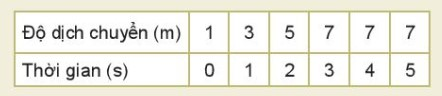
\includegraphics[scale=1]{../figs/VN10-2022-PH-TP006-3.jpg}
		\end{center}
		
		Dựa vào bảng để:
		
		\begin{enumerate}[label=\alph*)]
			\item Vẽ đồ thị độ dịch chuyển - thời gian của chuyển động.
			\item Mô tả chuyển động của xe.
			\item Tính vận tốc của xe trong $\SI{3}{s}$ đầu.
		\end{enumerate}
	}
	\hideall{
		
		\begin{enumerate}[label=\alph*)]
			\item Vẽ đồ thị độ dịch chuyển - thời gian của chuyển động
			
			\begin{center}
				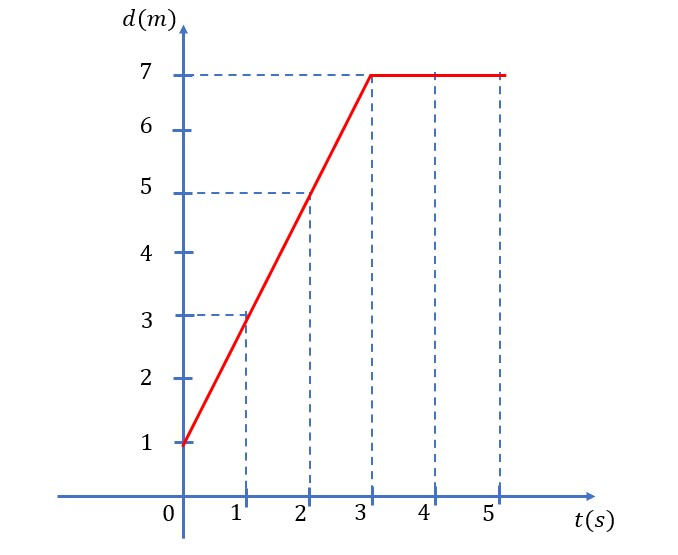
\includegraphics[scale=0.6]{../figs/VN10-2022-PH-TP006-7.jpg}
			\end{center}
			
			\item Mô tả chuyển động của xe
			
			- Từ 0 – 3 giây: xe chuyển động thẳng.
			
			- Từ giây thứ 3 đến giây thứ 5: xe đứng yên (dừng lại).
			
			
			\item 
			Độ dịch chuyển của xe trong 3 giây đầu là:
			
			$$d = 7-1 = \SI{6}{m}.$$
			
			Vận tốc của xe trong $\SI{3}{s}$ đầu
			
			$$v = \dfrac{\Delta d}{\Delta t} = \SI{2}{m/s}.$$
			
		\end{enumerate}
	}
	\item \mkstar{3}
	
	{
		Đồ thị độ dịch chuyển - thời gian trong chuyển động thẳng của một xe ô tô đồ chơi điều khiển từ xa được vẽ ở hình: 
		\begin{center}
			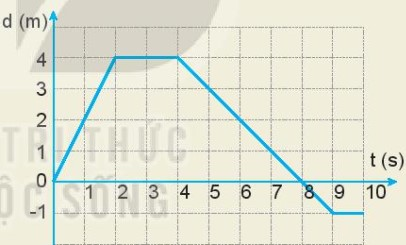
\includegraphics[scale=1]{../figs/VN10-2022-PH-TP006-4.jpg}
		\end{center}
		
		
		\begin{enumerate}[label=\alph*)]
			\item Mô tả chuyển động của xe.
			\item Xác định vị trí của xe so với điểm xuất phát của xe ở giây thứ 2, giây thứ 4, giây thứ 8 và giây thứ 10.
			\item Xác định tốc độ và vận tốc của xe trong 2 giây đầu, từ giây 2 đến giây 4 và từ giây 4 đến giây 8.
			\item Xác định quãng đường đi được và độ dịch chuyển của xe sau 10 giây chuyển động. Tại sao giá trị của chúng không giống nhau?
		\end{enumerate}
	}
	\hideall{
		
		\begin{enumerate}[label=\alph*)]
			\item Mô tả chuyển động của xe
			
			- Trong 2 giây đầu: xe chuyển động thẳng
			
			- Từ giây thứ 2 đến giây thứ 4: xe đứng yên
			
			- Từ giây thứ 4 đến giây thứ 10: xe chuyển động thẳng theo chiều ngược lại.
			
			- Từ giây thứ 9 đến giây thứ 10: xe dừng lại.
			
			\item 
			
			- Ở giây thứ 2: xe ở vị trí cách điểm xuất phát $\SI{4}{m}$.
			
			- Ở giây thứ 4: xe ở vị trí cách điểm xuất phát $\SI{4}{m}$.
			
			- Ở giây thứ 8: xe trở về vị trí xuất phát.
			
			- Ở giây thứ 10: xe ở vị trí cách điểm xuất phát $\SI{1}{m}$ theo chiều âm.
			\item Xác định tốc độ và vận tốc của xe
			
			- Trong 2 giây đầu, xe chuyển động thẳng, không đổi chiều nên tốc độ bằng vận tốc:
			
			$$v = \dfrac{d}{t} = \SI{2}{m/s}.$$
			
			- Từ giây 2 đến giây 4: xe đứng yên nên vận tốc và tốc độ của xe đều bằng 0.
			
			- Từ giây 4 đến giây 8:
			
			+ Tốc độ:
			
			$$v = \dfrac{s}{t} = \SI{1}{m/s}.$$
			
			+ Vận tốc:
			
			$$v = \dfrac{\Delta d}{\Delta t} = -\SI{1}{m/s}.$$
			\item
			- Từ đồ thị, ta thấy quãng đường đi được của xe sau 10 giây chuyển động là:
			
			$$s = 4 + 4 + 1 = \SI{9}{m}.$$
			
			- Độ dịch chuyển của xe sau 10 giây là:
			
			$$d = - 1 - 4 + 4 = - \SI{1}{m}.$$
			
			Suy ra quãng đường và độ dịch chuyển của xe sau 10 giây không giống nhau vì xe chuyển động theo 2 chiều.
		\end{enumerate}
	}
	
\end{enumerate}